\documentclass[10pt]{beamer}

\usepackage[utf8]{inputenc}
\usepackage[spanish, es-tabla]{babel}

\usetheme{metropolis}
\usepackage{appendixnumberbeamer}

\usepackage{booktabs}
\usepackage[scale=2]{ccicons}

\usepackage{pgfplots}
\usepgfplotslibrary{dateplot}

\usepackage{caption}
\usepackage{subcaption}
\usepackage{tabulary}

\usepackage{graphicx}

\usepackage[normalem]{ulem}
\useunder{\uline}{\ul}{}

\usepackage{amsmath}
\usepackage{amsfonts}
\usepackage{amssymb}
\usepackage{amsthm}
\usepackage{esvect}

\usepackage{multimedia}

\usepackage[spanish,onelanguage]{algorithm2e} %for psuedo code

\usepackage{xspace}
\newcommand{\themename}{\textbf{\textsc{metropolis}}\xspace}

\title{Detección de anomalías en Series Temporales mediante uso de técnicas Deep Learning}
\author{Ignacio Aguilera Martos}
\date{10 Septiembre 2020}
\institute{Trabajo Fin de Máster \\ \href{https://github.com/nacheteam/DLOD}{Código disponible en GitHub}}

\begin{document}

\maketitle

\begin{frame}[fragile]{Contenidos}
  \setbeamertemplate{section in toc}[sections numbered]
  %\tableofcontents[hideallsubsections]
  \tableofcontents
\end{frame}

\section{Contenido teórico}

\begin{frame}[fragile]{Contenido teórico de la memoria}
	\vspace{10px}
	\pause
	\metroset{block=fill}
	
	\begin{block}{Contenido teórico tratado}
		\begin{enumerate}
			\item Machine Learning: aprendizaje, regularización y cotas del aprendizaje.
			\pause
			\item Estadística Multivariante: independencia, probabilidad y esperanza condicionadas, desigualdades famosas.
			\pause
			\item Redes Neuronales y Deep Learning: aprendizaje, capas empleadas y Autoencoders.
		\end{enumerate}
	\end{block}
	
\end{frame}

\subsection{Conceptos de anomalía}

\begin{frame}[fragile]{Concepto de anomalía}
	\vspace{10px}
	\pause
	\metroset{block=fill}
	
	\begin{block}{Tukey's Fences}
		Valores fuera del rango $[Q_1 - k(Q_3 - Q_1), Q_3 + k(Q_3 - Q_1)]$ con $k=$1.5, 3, 5
		
		No podemos aplicarlo directamente a varias dimensiones.
	\end{block}

	\pause

	\begin{block}{Criterio de clusters}
		\begin{enumerate}
			\item Agrupamos los datos por clusters.
			\pause
			\item Encontramos el cluster más cercano para cada instancia.
			\pause
			\item Si la distancia del objeto al centroide del cluster es mayor que $1.5$ veces la mayor
			distancia intercluster entonces es una anomalía.
		\end{enumerate}
	\end{block}
	
\end{frame}

\begin{frame}[fragile]{Ejemplo 1}
	\vspace{10px}
	\metroset{block=fill}
	\centering
	\movie[height = 0.8\textheight, width=0.8\textwidth, poster, showcontrols]{}{Imagenes/outlier-2d-case1.mp4}
	
\end{frame}

\begin{frame}[fragile]{Ejemplo 1}
	\vspace{10px}
	\metroset{block=fill}
	
	\begin{figure}
		\centering
		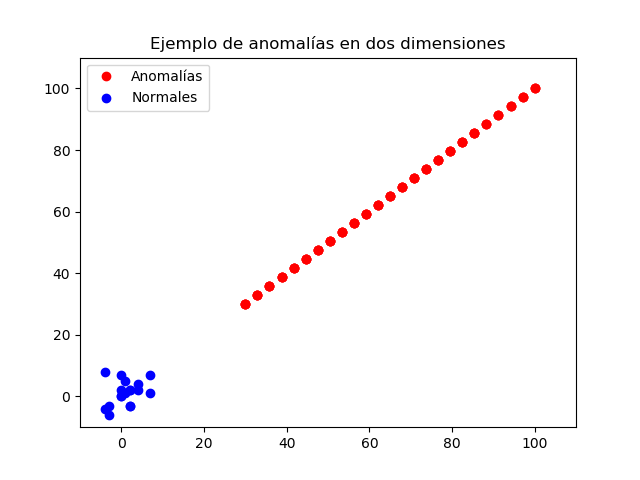
\includegraphics[scale=0.6]{Imagenes/outlier-2d-case1.png}
	\end{figure}
	
\end{frame}

\begin{frame}[fragile]{Ejemplo 2}
	\vspace{10px}
	\metroset{block=fill}
	\centering
	\movie[height = 0.8\textheight, width=0.8\textwidth, poster, showcontrols]{}{Imagenes/outlier-2d-case2.mp4}
	
\end{frame}

\begin{frame}[fragile]{Ejemplo 2}
	\vspace{10px}
	\metroset{block=fill}
	
	\begin{figure}
		\centering
		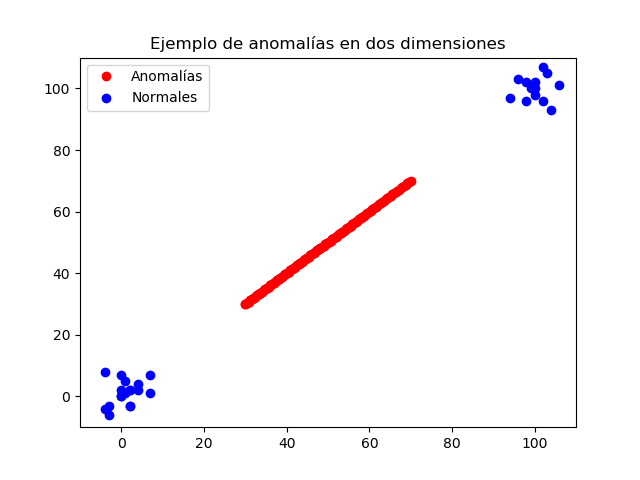
\includegraphics[scale=0.6]{Imagenes/outlier-2d-case2.png}
	\end{figure}
	
\end{frame}

\subsection{Concepto de anomalía probabilístico}


\begin{frame}[fragile]{Notación}
	\vspace{10px}
	\pause
	\metroset{block=fill}
	
	\begin{block}{Notación usada}
		$$X = \{ x_1 , ... , x_n \}, \ x_i = (x_{s_1} , ... , x_{s_d})$$
		
		\pause
		
		$$S = \{ s_i | s_i \in \{ s_1 , ... , s_d \} \ con \ i\in \Delta \}$$
		
		\pause
		
		$$X_S \ proyecci\acute{o}n \ de \ los \ datos \ en \ el \ subespacio \ S$$
		
		\pause
		
		$$p_{s_1 , ... , s_p}(x_{s_1} , ... , x_{s_p})$$
		
		\pause
		
		$$p_{s_i}(x_{s_i})$$
	\end{block}
	
\end{frame}

\begin{frame}[fragile]{Definiciones}
	\vspace{10px}
	\pause
	\metroset{block=fill}
	
	\begin{block}{Definición subespacio incorrelado}
		Decimos que un subespacio $S$ es un subespacio incorrelado si y sólo si:
		
		$$p_{s_1 , ... , s_p}(x_{s_1} , ... , {x_{s_p}}) = \prod_{i=1}^{p}p_{s_i}(x_{s_i})$$
	\end{block}
	
	\pause
	
	\begin{block}{Definición anomalía no trivial}
		Decimos que un objeto $x_S$ es una anomalía no trivial respecto del subespacio $S$ si:
		
		$$p_{s_1 , ... , s_p}(x_{s_1} , ... , x_{s_p})\ll p_{esp}(x_{s_1} , ... , x_{s_p})$$
	\end{block}
	
	\pause
	
	\begin{alertblock}{Relación entre conceptos de anomalía}
		Este concepto de anomalía es complementario.
	\end{alertblock}
	
\end{frame}

\begin{frame}[fragile]{Ejemplo de anomalía probabilística}
	\vspace{10px}
	\pause
	\metroset{block=fill}
	
	\begin{figure}
		\centering
		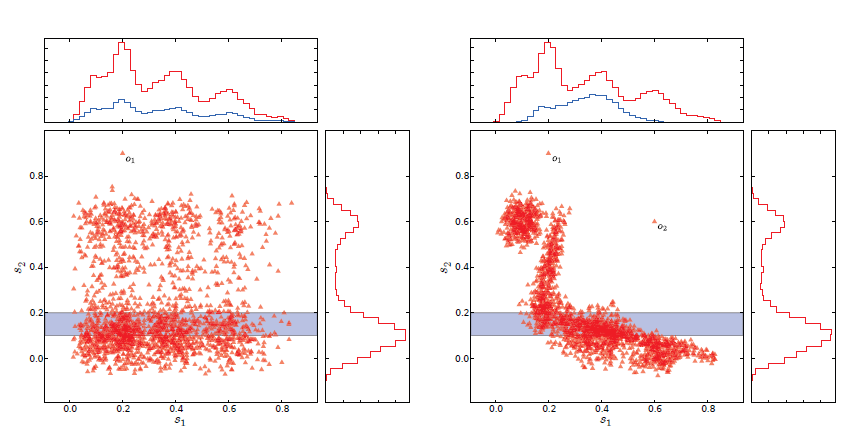
\includegraphics[scale=0.5]{Imagenes/ejemplo_anomalia_probabilidad}
	\end{figure}
	
\end{frame}

\section{Explicación del problema}

\begin{frame}[fragile]{Explicación del problema}
	\vspace{10px}
	\pause
	\metroset{block=fill}
	
	\begin{block}{Definición del problema}
		La empresa ArcelorMittal tiene una máquina sobre la que quiere detectar los mantenimientos antes de que ocurran.
		
		Tenemos una serie temporal de 468 días con medidas cada un segundo y 106 variables en total.
		
		Empleamos 438 como entrenamiento, 30 para hallar cotas y 30 para test, dejando más de 2.5 millones de instancias en test.
	\end{block}

	\begin{exampleblock}{Enfoque}
		Obtenemos las puntuaciones de anomalías con algoritmos para ello, luego obtenemos una clasificación de los puntos y finalmente los pasamos por un sistema de alertas basado en ventanas.
	\end{exampleblock}
	
\end{frame}

\begin{frame}[fragile]{Algoritmo de alarmas}
	\vspace{10px}
	\pause
	\metroset{block=fill}
	
	Calculamos las puntuaciones con un método de detección de anomalías.
	
	Pasamos una ventana deslizante y calculamos una cota local, hacemos la media con la cota general y comprobamos si la puntuación es mayor que la combinación de las cotas.
	
	Sobre los datos clasificados pasamos ventanas deslizantes y comprobamos si hay más de un 5\% de anomalías, entonces damos alerta.
	
\end{frame}

\section{Modelos implementados}

\begin{frame}[fragile]{Modelos de detección de anomalías}
	\vspace{10px}
	\pause
	\metroset{block=fill}
	
	\begin{block}{Tipos de modelos}
		Modelos Autoencoder: codifican y reconstruyen las instancias. A peor reconstrucción más anómalo es el dato.
		
		Modelos de Predicción: aprenden a predecir en condiciones de normalidad. Cuanto peor lo hagan más anómalo será el dato.
	\end{block}
	
\end{frame}

\begin{frame}[fragile]{Modelos Deep Learning implementados}
	\vspace{10px}
	\pause
	\metroset{block=fill}
	
	\begin{block}{Modelos}
		\begin{itemize}
			\item Autoencoder totalmente conectado simétrico.
			\pause
			\item Autoencoder totalmente conectado simétrico por lotes.
			\pause
			\item Autoencoder con capas LSTM simétrico.
			\pause
			\item Predicción con capas LSTM.
			\pause
			\item Predicción con capas CNN-LSTM.
		\end{itemize}
	\end{block}
	
\end{frame}

\begin{frame}[fragile]{Autoencoder totalmente conectado}
	\vspace{10px}
	\pause
	\metroset{block=fill}
	
	\begin{figure}[H]
		\centering
		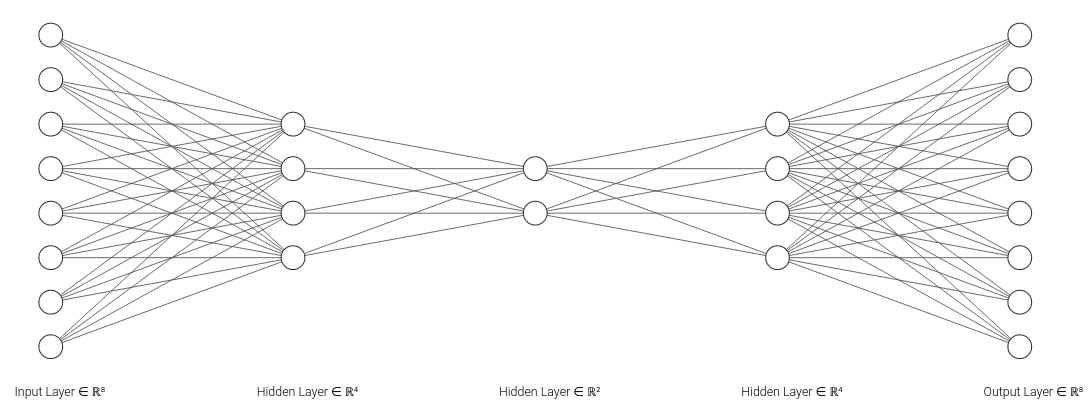
\includegraphics[scale=0.29]{Imagenes/autoencoder-fcc.png}
	\end{figure}
	
\end{frame}

\begin{frame}[fragile]{Autoencoder totalmente conectado por lotes}
	\vspace{10px}
	\pause
	\metroset{block=fill}
	
	\begin{figure}[H]
		\centering
		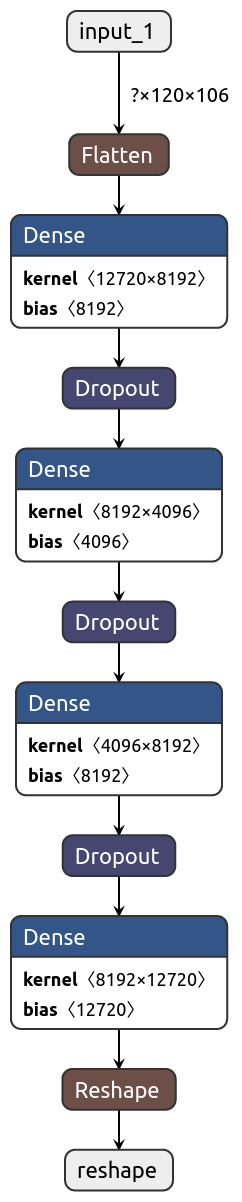
\includegraphics[scale=0.17]{Imagenes/autoencoder-fcc-batch.png}
	\end{figure}
	
\end{frame}

\begin{frame}[fragile]{Autoencoder LSTM}
	\vspace{10px}
	\pause
	\metroset{block=fill}
	
	\begin{figure}[H]
		\centering
		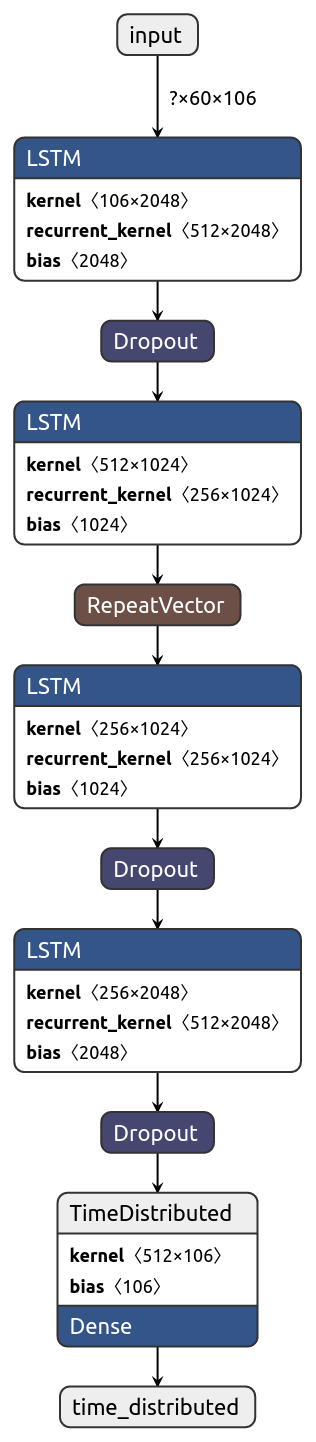
\includegraphics[scale=0.15]{Imagenes/autoencoder-lstm.png}
	\end{figure}
	
\end{frame}

\begin{frame}[fragile]{Predictor LSTM}
	\vspace{10px}
	\pause
	\metroset{block=fill}
	
	\begin{figure}[H]
		\centering
		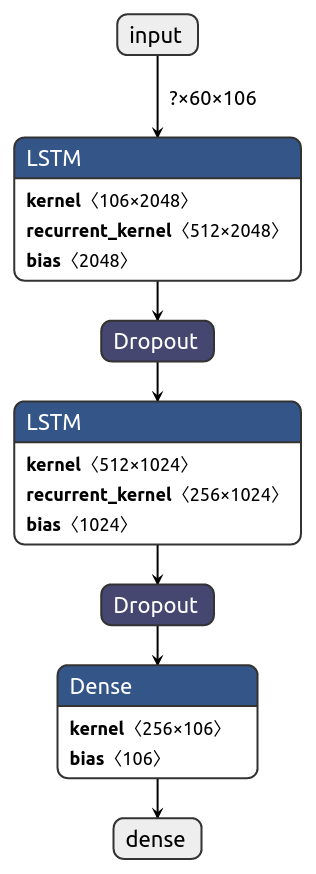
\includegraphics[scale=0.23]{Imagenes/lstm-forecaster.png}
	\end{figure}
	
\end{frame}

\begin{frame}[fragile]{Predictor CNN-LSTM}
	\vspace{10px}
	\pause
	\metroset{block=fill}
	
	\begin{figure}[H]
		\centering
		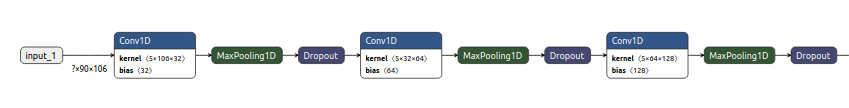
\includegraphics[scale=0.35]{Imagenes/cnn-lstm-forecaster-horizontal1.png}
	\end{figure}

	\begin{figure}[H]
		\centering
		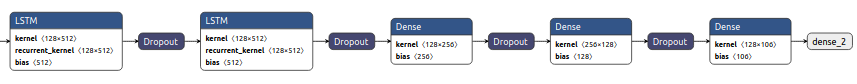
\includegraphics[scale=0.35]{Imagenes/cnn-lstm-forecaster-horizontal2.png}
	\end{figure}
	
\end{frame}

\section{Resultados obtenidos}

\begin{frame}[fragile]{Resultados iniciales}
	\vspace{10px}
	\pause
	\metroset{block=fill}
	
	\begin{table}[H]
		\centering
		\begin{tabulary}{\textwidth}{|l|c|c|c|c|c|c|}
			\hline
			\multicolumn{1}{|c|}{\textbf{Modelo}} & \textbf{TP} & \textbf{FP} & \textbf{TN}  & \textbf{FN} & \textbf{M.D.} & \textbf{M.T.} \\ \hline
			\textbf{AE FCC}                       & 33          & 441         & 75           & 8           & 20            & 28            \\ \hline
			\textbf{AE FCC lotes}                 & 33          & 393         & 123          & 8           & 20            & 28            \\ \hline
			\textbf{AE LSTM}                      & 33          & 447         & 69           & 8           & 20            & 28            \\ \hline
			\textbf{Predictor LSTM}               & 33          & 393         & 123          & 8           & 20            & 28            \\ \hline
			\textbf{Predictor CNN-LSTM}           & 35          & 213         & 301          & 8           & 22            & 28            \\ \hline
			\textbf{FB LOF}                       & 15          & \textbf{56} & \textbf{340} & 20          & 8             & 28            \\ \hline
			\textbf{HBOS}                         & \textbf{44} & 505         & 0            & \textbf{5}  & \textbf{23}   & 28            \\ \hline
			\textbf{IForest}                      & 28          & 344         & 177          & 9           & 19            & 28            \\ \hline
			\textbf{KNN}                          & 42          & 505         & 1            & \textbf{5}  & \textbf{23}   & 28            \\ \hline
			\textbf{LODA}                         & 36          & 341         & 172          & 6           & 22            & 28            \\ \hline
			\textbf{LOF}                          & 40          & 471         & 38           & 6           & 22            & 28            \\ \hline
			\textbf{PCA}                          & 26          & 256         & 267          & 12          & 16            & 28            \\ \hline
		\end{tabulary}
	\end{table}
	
\end{frame}

\begin{frame}[fragile]{Porcentajes de acierto}
	\vspace{10px}
	\pause
	\metroset{block=fill}
	
	\begin{table}[H]
		\centering
		\begin{tabulary}{\textwidth}{|l|c|c|}
			\hline
			\multicolumn{1}{|c|}{\textbf{Modelo}} & \textbf{\begin{tabular}[c]{@{}c@{}}Tasa mantenimientos\\ detectados\end{tabular}} & \textbf{\begin{tabular}[c]{@{}c@{}}Acierto sobre\\ ventanas\end{tabular}} \\ \hline
			\textbf{AE FCC}                       & 0.7143                                                                            & 0.1939                                                                    \\ \hline
			\textbf{AE FCC lotes}                 & 0.7143                                                                            & 0.2801                                                                    \\ \hline
			\textbf{AE LSTM}                      & 0.7143                                                                            & 0.1831                                                                    \\ \hline
			\textbf{Predictor LSTM}               & 0.7143                                                                            & 0.2801                                                                    \\ \hline
			\textbf{Predictor CNN-LSTM}           & 0.7857                                                                            & 0.6054                                                                    \\ \hline
			\textbf{FB LOF}                       & 0.2857                                                                            & \textbf{0.8237}                                                           \\ \hline
			\textbf{HBOS}                         & \textbf{0.8214}                                                                   & 0.0794                                                                    \\ \hline
			\textbf{IForest}                      & 0.6786                                                                            & 0.3674                                                                    \\ \hline
			\textbf{KNN}                          & \textbf{0.8214}                                                                   & 0.0794                                                                    \\ \hline
			\textbf{LODA}                         & 0.7857                                                                            & 0.3748                                                                    \\ \hline
			\textbf{LOF}                          & 0.7857                                                                            & 0.1405                                                                    \\ \hline
			\textbf{PCA}                          & 0.5714                                                                            & 0.5223                                                                    \\ \hline
		\end{tabulary}
	\end{table}
	
\end{frame}

\begin{frame}[fragile]{TPR, TNR, F1 y AUC}
	\vspace{10px}
	\pause
	\metroset{block=fill}
	
	\begin{table}[H]
		\centering
		\begin{tabulary}{\textwidth}{|l|c|c|c|c|c|}
			\hline
			\multicolumn{1}{|c|}{\textbf{Modelo}} & \textbf{TPR}    & \textbf{TNR}    & \textbf{TPRxTNR} & \textbf{F1}     & \textbf{AUC}  \\ \hline
			\textbf{AE FCC}                       & 0.8049          & 0.1453          & 0.1170           & 0.1282          & 0.48          \\ \hline
			\textbf{AE FCC lotes}                 & 0.8049          & 0.2384          & 0.1919           & 0.1413          & 0.52          \\ \hline
			\textbf{AE LSTM}                      & 0.8049          & 0.1337          & 0.1076           & 0.1267          & 0.47          \\ \hline
			\textbf{Pred. LSTM}               & 0.8049          & 0.2384          & 0.1919           & 0.1413          & 0.52          \\ \hline
			\textbf{Pred. CNN-LSTM}           & 0.8537          & 0.5856          & 0.5              & 0.2422          & 0.72          \\ \hline
			\textbf{FB LOF}                       & 0.4286          & \textbf{0.8586} & \textbf{0.3680}  & 0.2830          & 0.64          \\ \hline
			\textbf{HBOS}                         & \textbf{0.8980} & 0               & 0                & \textbf{0.1471} & \textbf{0.45} \\ \hline
			\textbf{IForest}                      & 0.7568          & 0.3397          & 0.2571           & 0.1369          & 0.55          \\ \hline
			\textbf{KNN}                          & 0.8959          & 0.0020          & 0.0018           & \textbf{0.1443} & \textbf{0.45} \\ \hline
			\textbf{LODA}                         & 0.8571          & 0.3353          & 0.2874           & 0.1718          & 0.6           \\ \hline
			\textbf{LOF}                          & 0.8696          & 0.0747          & 0.0649           & 0.1436          & 0.47          \\ \hline
			\textbf{PCA}                          & 0.6842          & 0.5105          & 0.3493           & 0.1625          & 0.6           \\ \hline
		\end{tabulary}
	\end{table}
	
\end{frame}

\begin{frame}[fragile]{ROC de los mejores modelos}
	\pause
	\metroset{block=fill}
	
	\begin{figure}[H]
		\centering
		\begin{subfigure}{.49\textwidth}
			\centering
			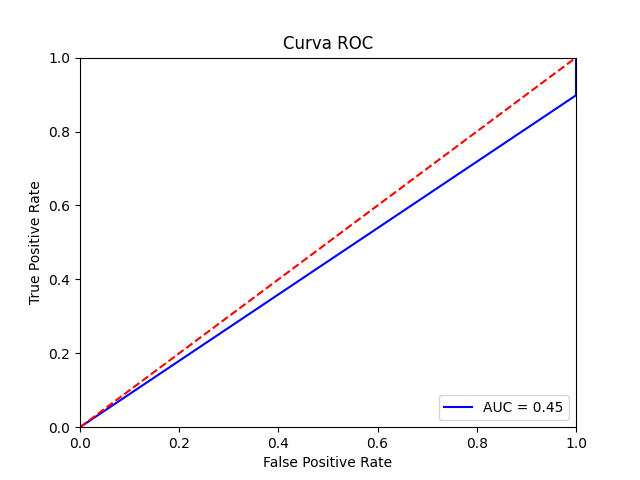
\includegraphics[scale=0.27]{Imagenes/HBOS_roc.png}
			\caption{Curva ROC HBOS.}
		\end{subfigure}
		\begin{subfigure}{.49\textwidth}
			\centering
			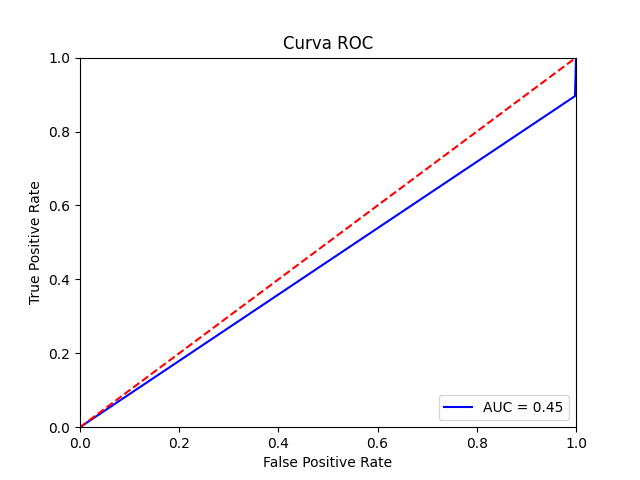
\includegraphics[scale=0.27]{Imagenes/KNN_roc.png}
			\caption{Curva ROC KNN.}
		\end{subfigure}
	\end{figure}

	\begin{figure}[H]
		\centering
		\begin{subfigure}{.49\textwidth}
			\centering
			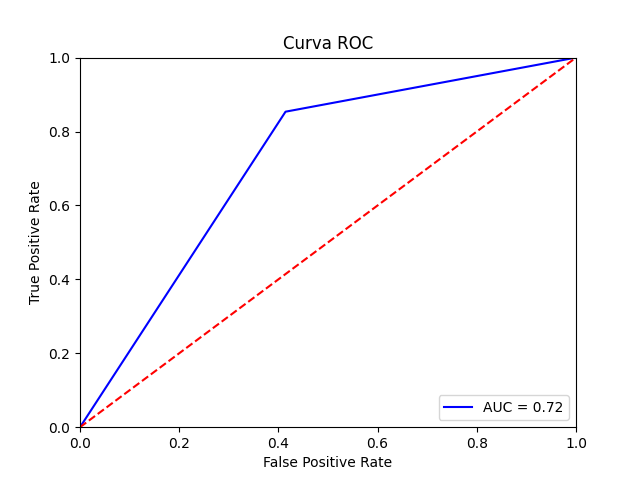
\includegraphics[scale=0.27]{Imagenes/Predictor-CNN-LSTM_roc.png}
			\caption{Curva ROC Predictor CNN-LSTM.}
		\end{subfigure}
		\begin{subfigure}{.49\textwidth}
			\centering
			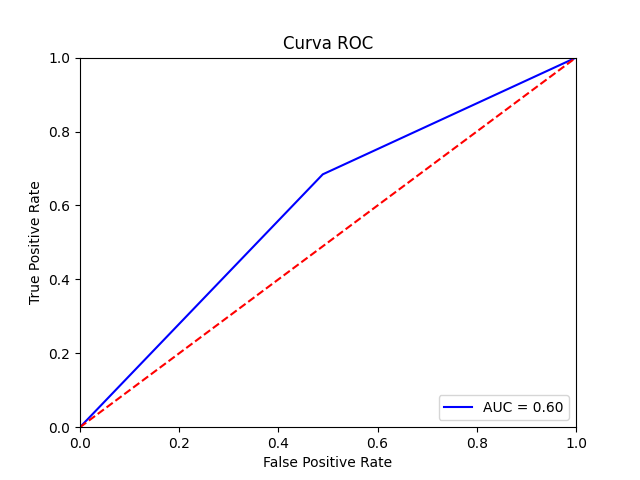
\includegraphics[scale=0.27]{Imagenes/PCA_roc.png}
			\caption{Curva ROC PCA.}
		\end{subfigure}
	\end{figure}
	
\end{frame}

\begin{frame}[fragile]{Tiempos entrenamiento}
	\vspace{10px}
	\pause
	\metroset{block=fill}
	
	\begin{figure}[H]
		\centering
		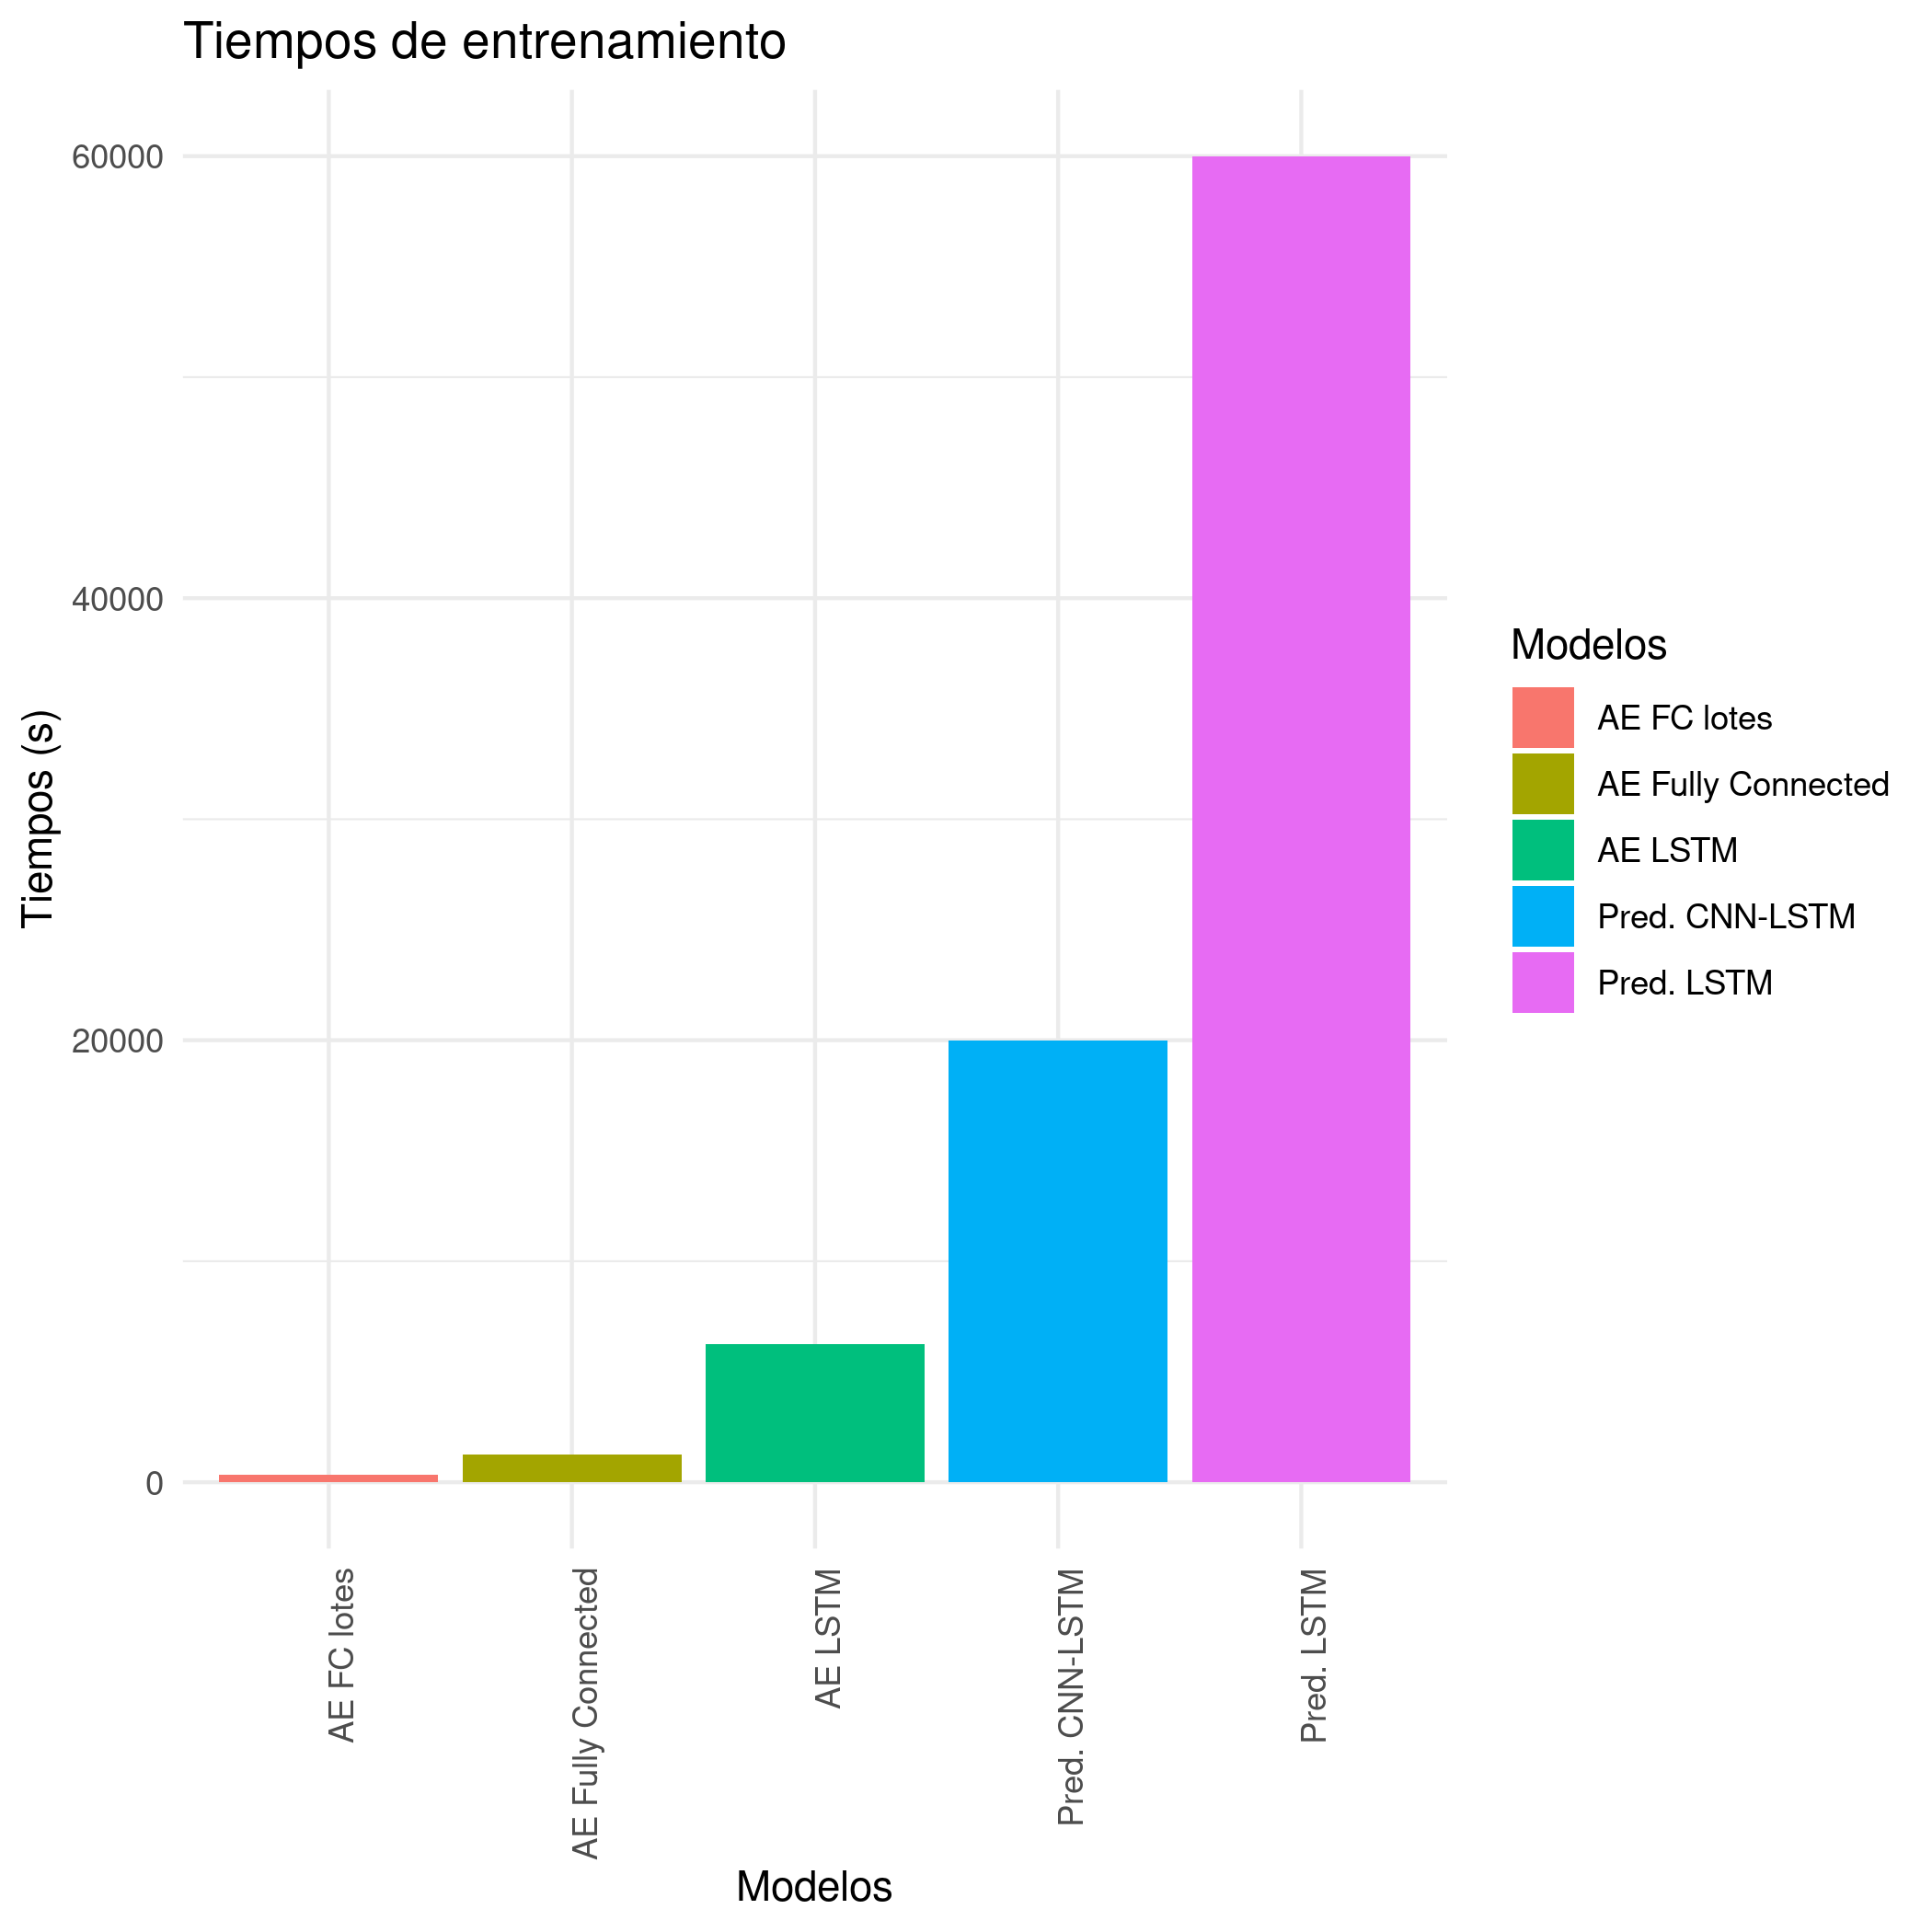
\includegraphics[scale=0.43]{Imagenes/tiempos_entrenamiento.png}
	\end{figure}
	
\end{frame}

\begin{frame}[fragile]{Tiempos de predicción}
	\vspace{10px}
	\pause
	\metroset{block=fill}
	
	\begin{figure}[H]
		\centering
		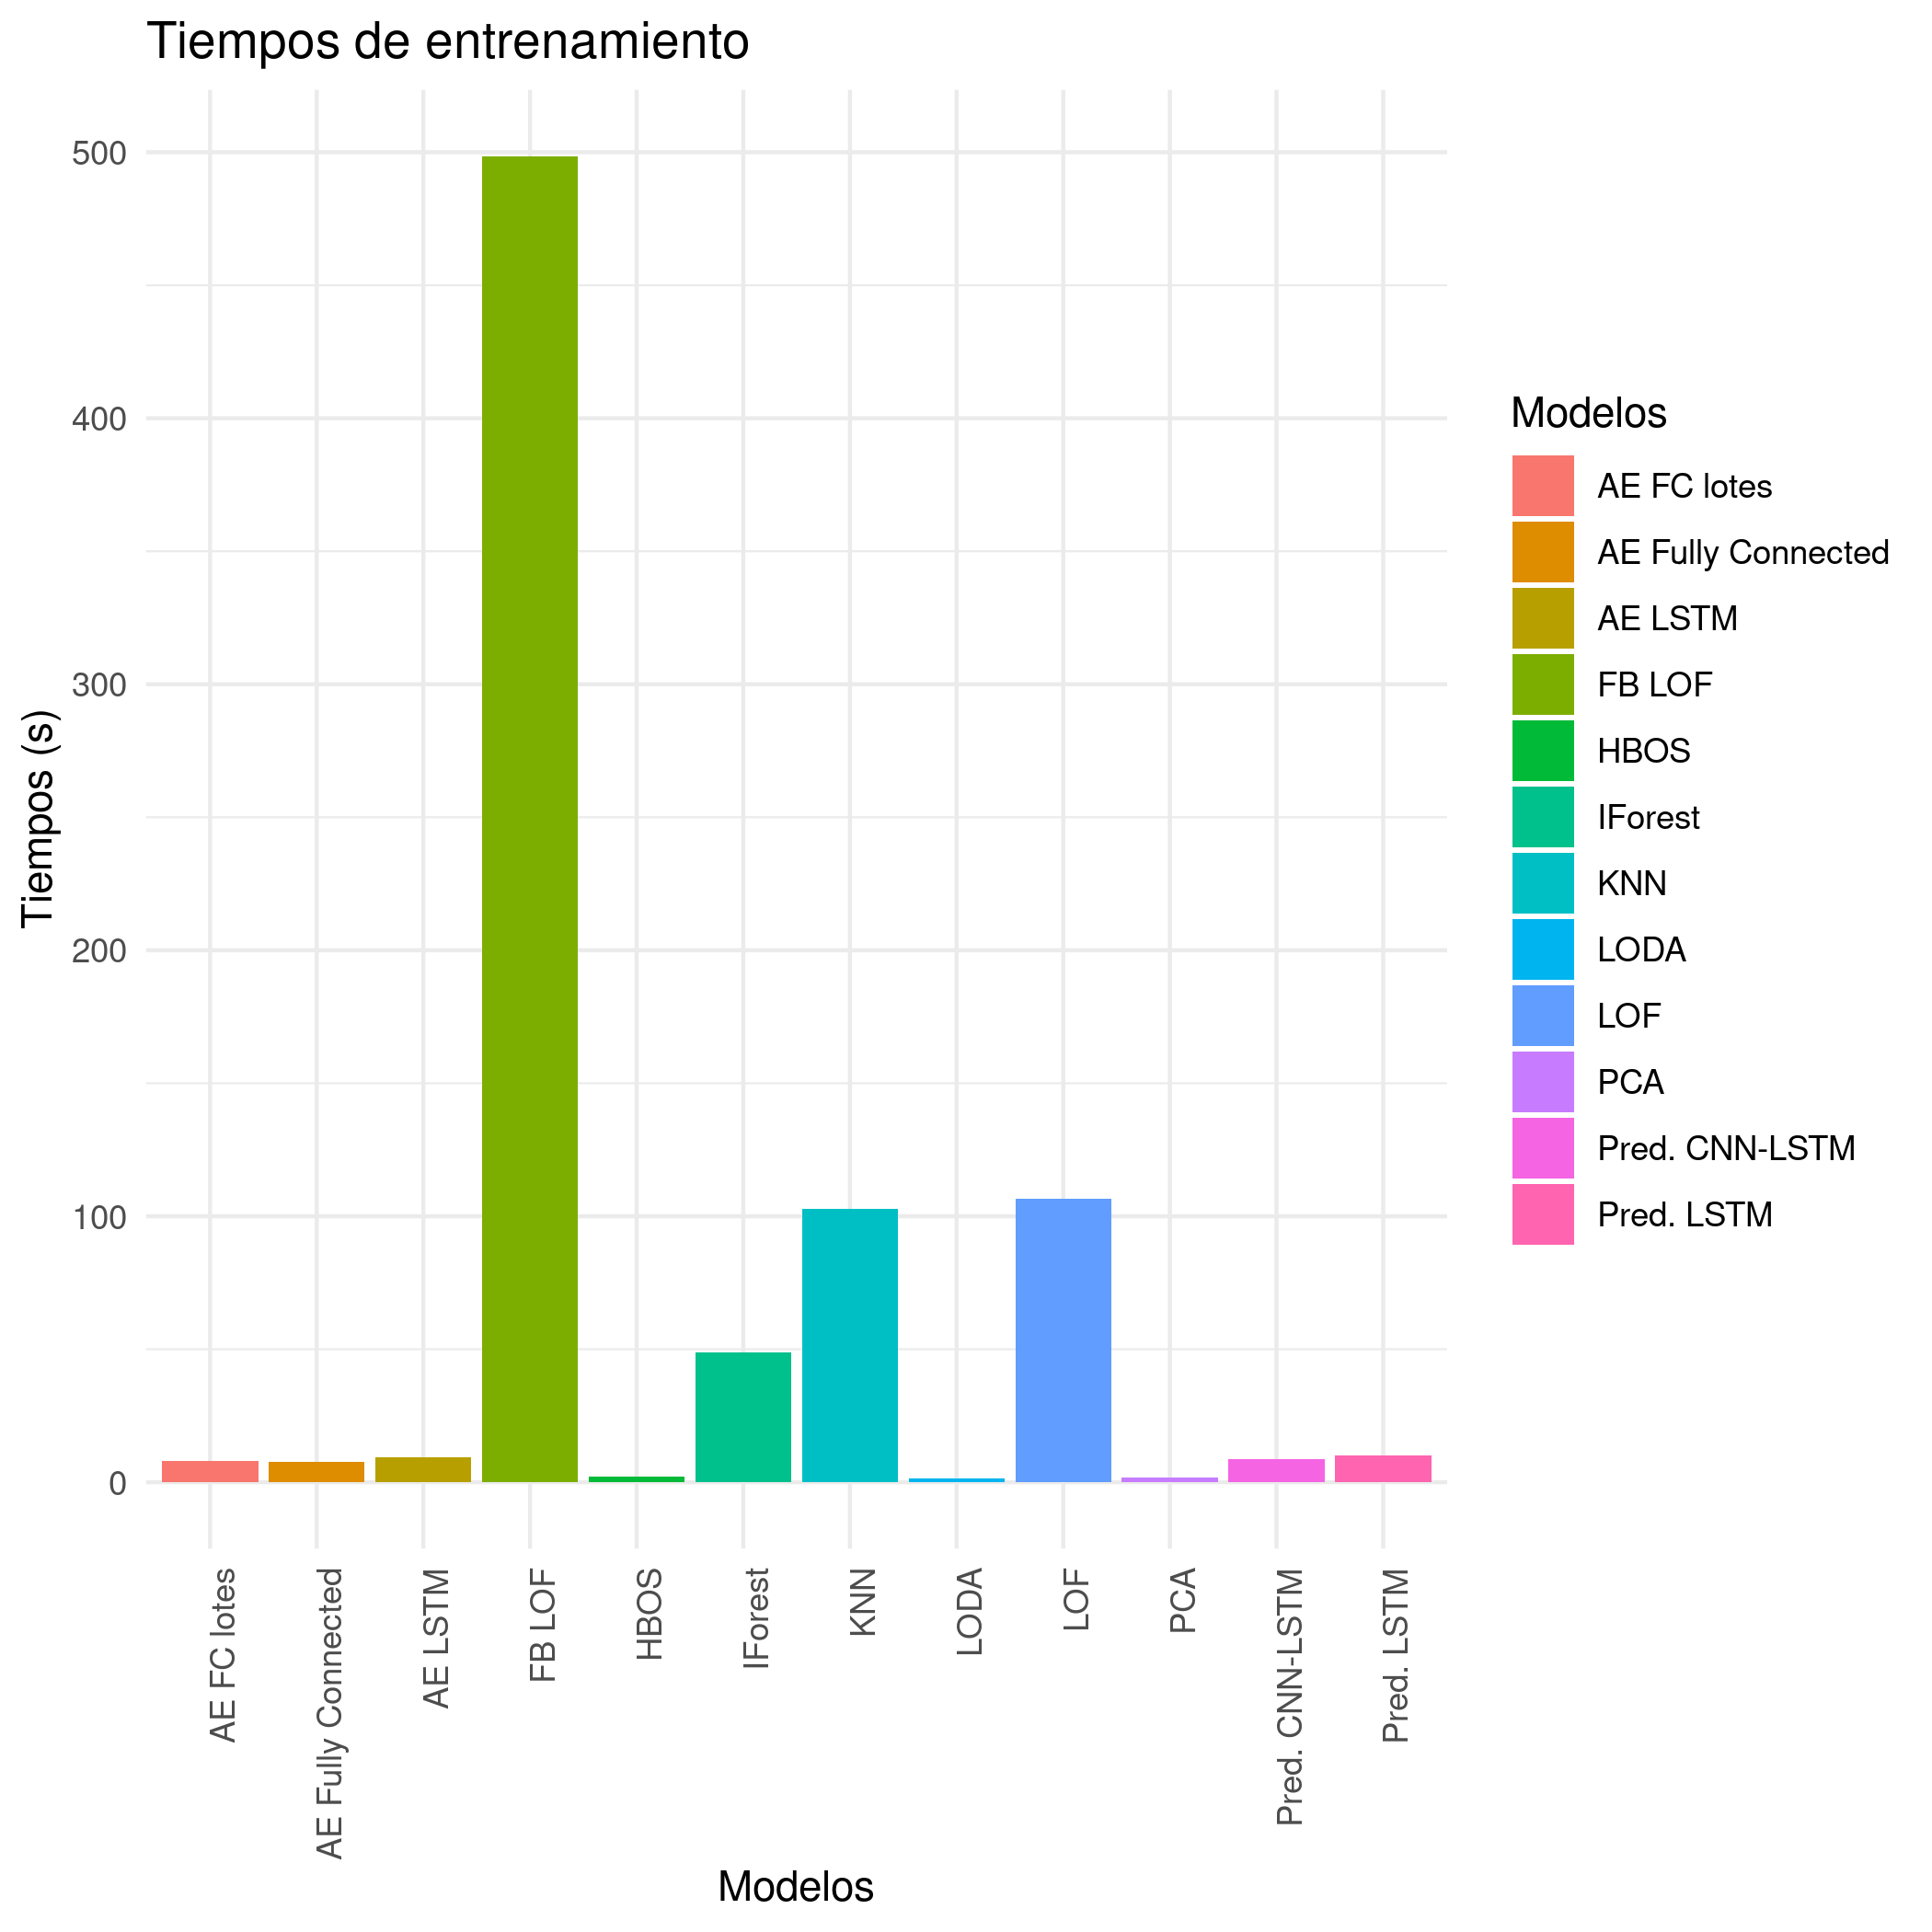
\includegraphics[scale=0.43]{Imagenes/tiempos_prediccion.png}
	\end{figure}
	
\end{frame}

\begin{frame}[fragile]{Tiempos de predicción}
	\vspace{10px}
	\pause
	\metroset{block=fill}
	
	\begin{figure}[H]
		\centering
		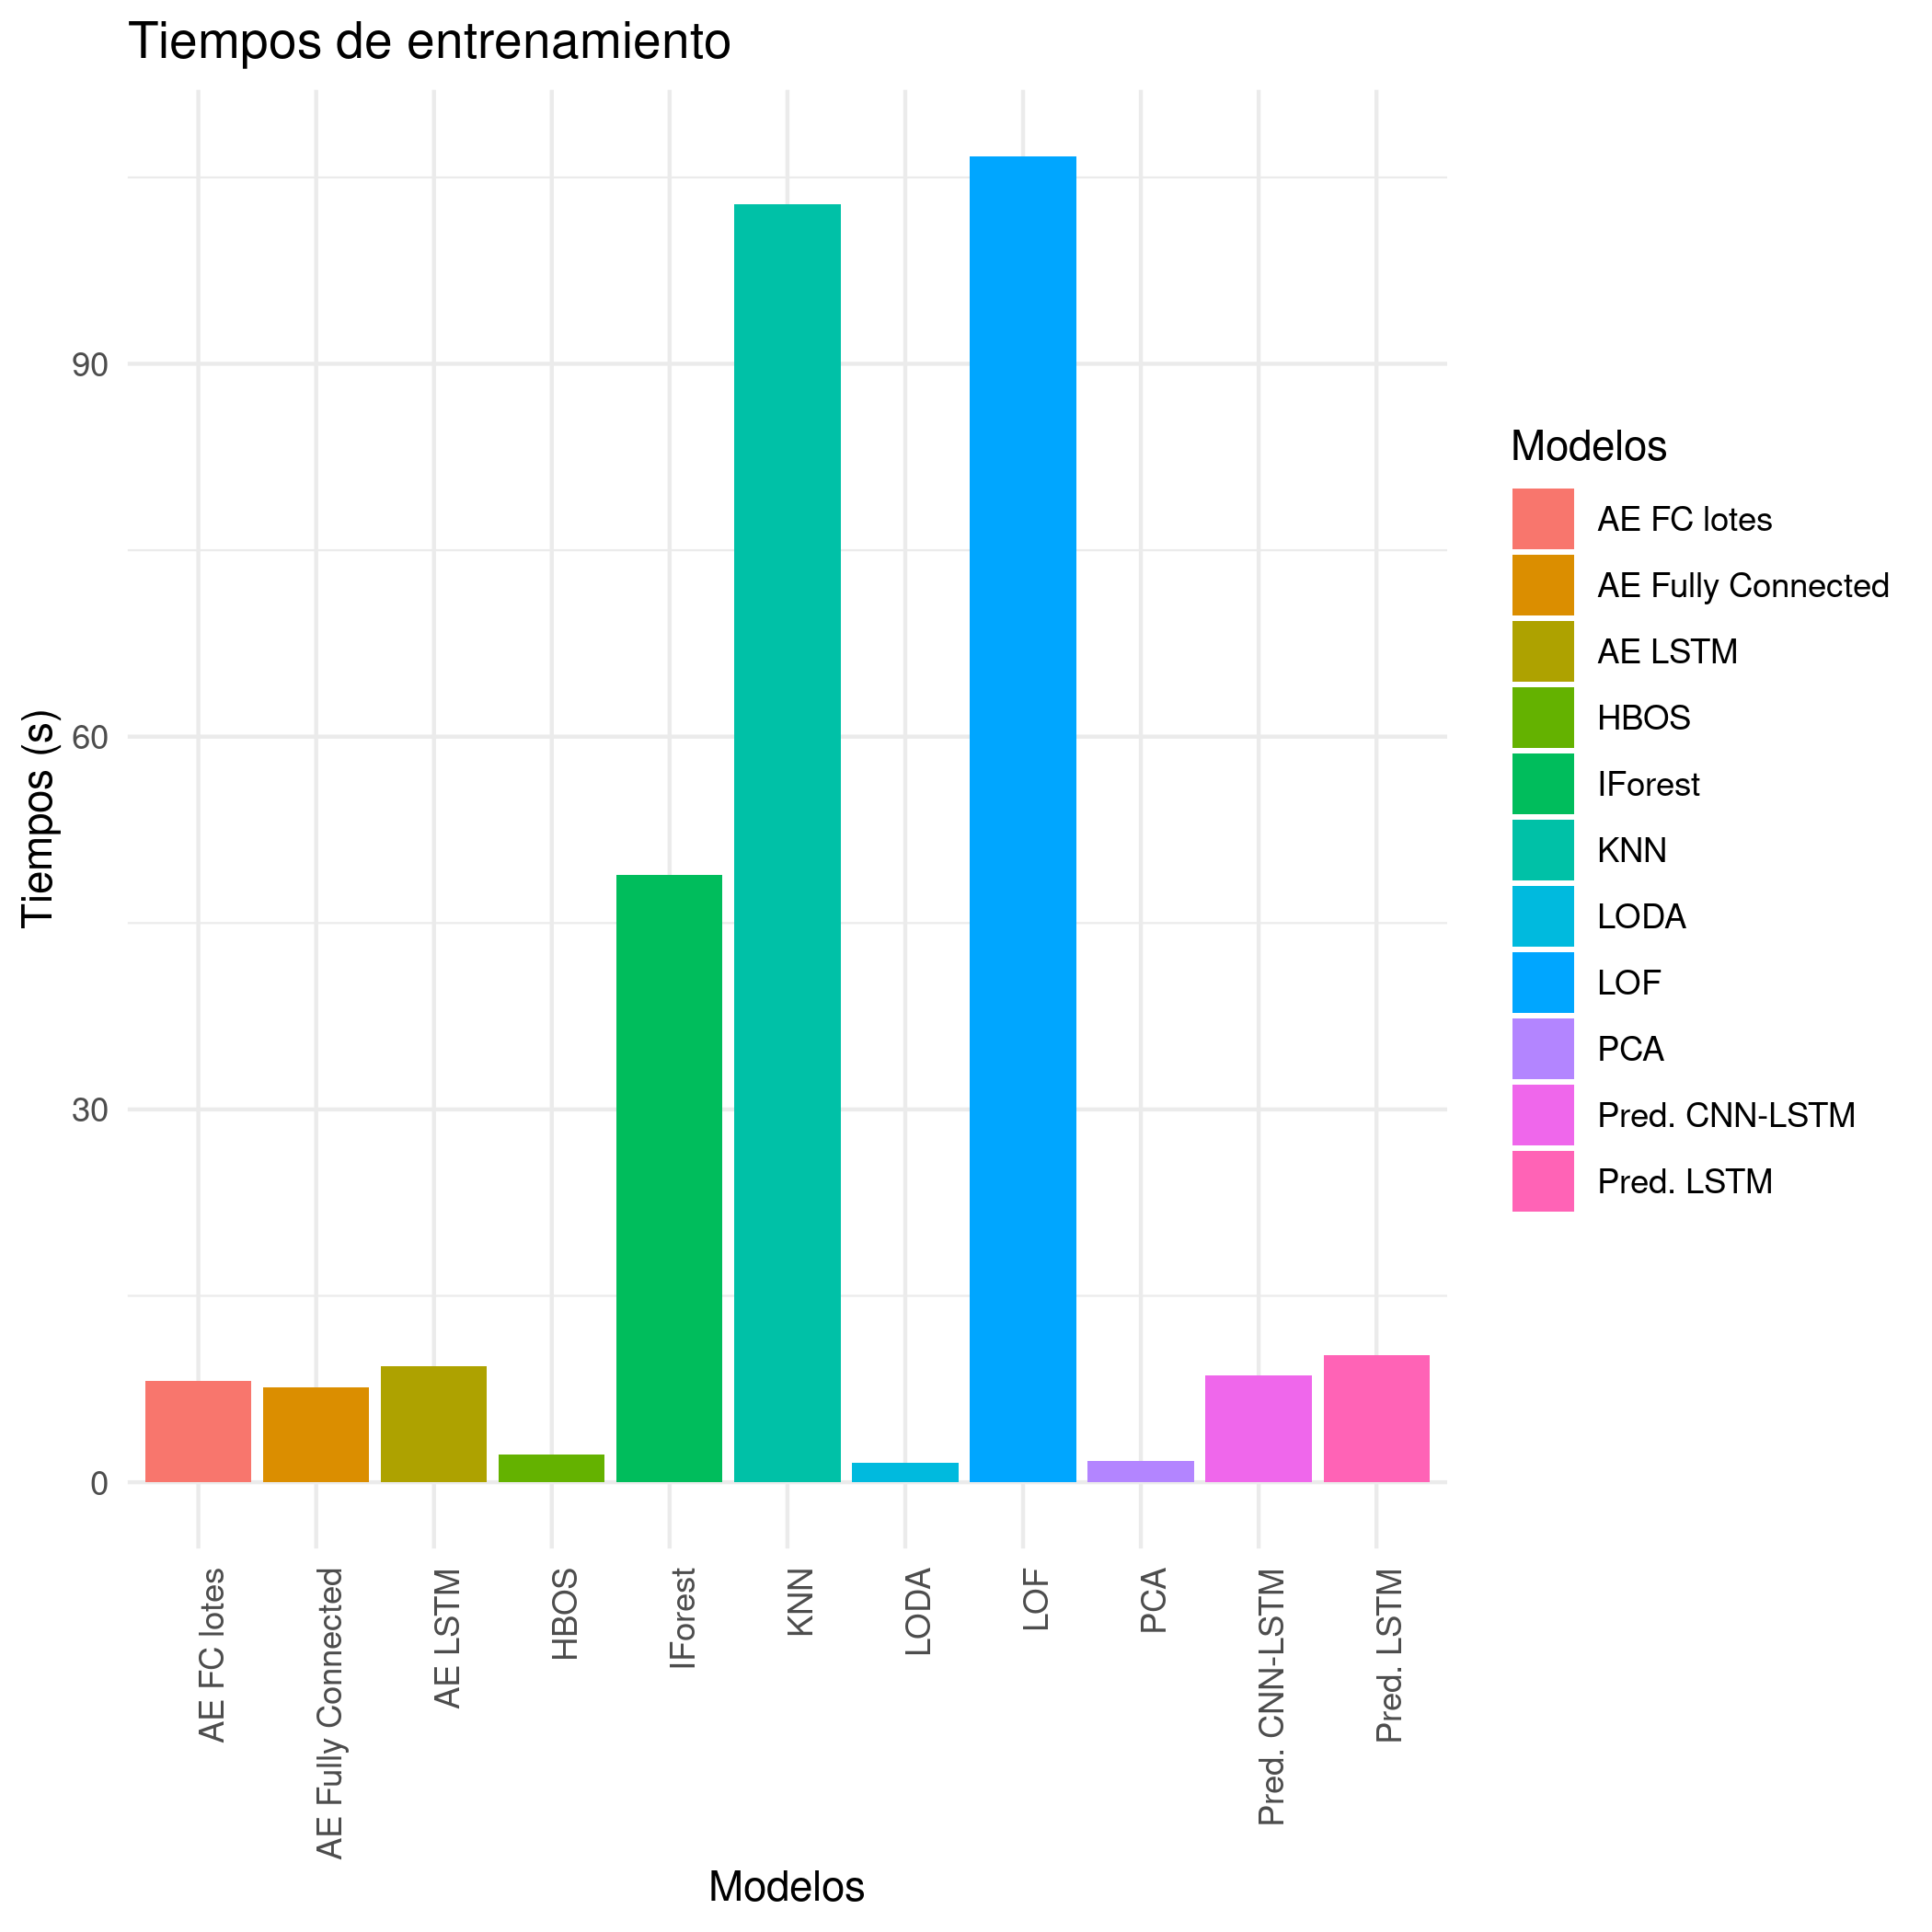
\includegraphics[scale=0.43]{Imagenes/tiempos_prediccion2.png}
	\end{figure}
	
\end{frame}

\section{Conclusiones y Trabajo Futuro}

\begin{frame}[fragile]{Conclusiones}
	\vspace{10px}
	\pause
	\metroset{block=fill}
	
	\begin{itemize}
		\item El modelo más equilibrado y el mejor es el modelo de predicción CNN-LSTM
		\pause
		\item Los modelos Deep Learning han demostrado gran potencial en la detección de anomalías.
		\pause
		\item Los modelos HBOS y KNN han dado buenos resultados como modelos clásicos.
		\pause
		\item Los modelos de predicción resultan mejores que los Autoencoder.
		\pause
		\item El algoritmo de clasificación de anomalías y detección de eventos anómalos es crucial.
		\pause
		\item Utilidad del estudio en su aplicación en el mundo real.
	\end{itemize}
	
\end{frame}

\begin{frame}[fragile]{Trabajo Futuro}
	\vspace{10px}
	\pause
	\metroset{block=fill}
	
	\begin{itemize}
		\item Empleo de técnicas de reducción de falsos positivos.
		\pause
		\item Búsqueda de los mejores parámetros para los modelos.
		\pause
		\item Añadir más arquitecturas Deep Learning a la comparativa.
		\pause
		\item Implementación de una arquitectura propia.
		\pause
		\item Implementar la metodología Test-Then-Train
		\pause
		\item Unir los TP, FP, TN y FN para analizarlos temporalmente.
	\end{itemize}
	
\end{frame}

\begin{frame}[standout]
	\LARGE{Gracias por su atención.}
	
	\vspace{10px}
	
	\LARGE{¿Preguntas?}
	\vspace{10px}
\end{frame}


\end{document}
